\documentclass[11pt,class=report,crop=false]{standalone}
\usepackage{exo7sv}

\begin{document}

%%%%%%%%%%%%%%%%%%%%%%%%%%%%%%%%%%%%%%%%%%%%%%%%%%%%%%%%%%%%%%%%%%%%%%
%%%%%%%%%%%%%%%%%%%%%%%%%%%%%%%%%%%%%%%%%%%%%%%%%%%%%%%%%%%%%%%%%%%%%%

\entete{Université de Lille}{Mathématiques pour la SVT}

\titre{Fiche 7. \quad Intégrales} 

\encadre{
\emph{Savoir.}
\begin{itemize}[label=$\square$]
  \item Comprendre le lien entre intégrale et aire.
  \item Connaître les propriétés de l'intégrale.
\end{itemize}
\emph{Savoir-faire.}
\begin{itemize}[label=$\square$]
  \item Savoir calculer des intégrales simples.
\end{itemize}
}

\insertvideo{epVYN8Py2zs}{Fiche 7. Intégrales}

\bigskip

%%%%%%%%%%%%%%%%%%%%%%%%%%%%%%%%%%%%%%%%%%%%%%%%%%%
\subsection*{Intégrale et aire}

Soit $f : \Rr \to \Rr$ une fonction.
Nous définissons l'intégrale comme l'aire sous la courbe de $f$.

\begin{minipage}{0.45\textwidth}
$$\mathcal{A} = \int_a^b f(x)\,\dd x$$
\end{minipage}
\begin{minipage}{0.5\textwidth}
\shorthandoff{?;:!}
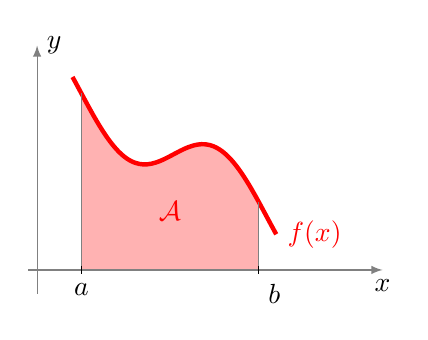
\begin{tikzpicture}[scale=1.5,xscale=1.5]
\tikzset{
	declare function={
		qcq(\t) = 1.5 - \t - 0.3*sin(6*(\t+1.05) r);
	}
}

 % tracé de la courbe et des axes
  \fill[red!30] (0,0) -- plot[domain=0:1] (\x,{qcq(\x)}) -- (1,0) -- cycle;
  \draw[ultra thick, color=red,domain=-0.05:1.1, smooth, samples=50] plot (\x,{qcq(\x)}) node[right] {$f(x)$};
  \draw[gray,->,>=latex] (-0.30,0) -- (1.7,0) node[below,black] {$x$};
  \draw[gray,->,>=latex] (-0.25,-0.2) -- (-0.25,1.9) node[right,black] {$y$};

  % tracé de la courbe par-dessus les rectangles
  % \draw[ultra thick, color=red,domain=-0.05:1.1, samples=100] plot (\x,{qcq(\x)}) node[right] {$y=f(x)$};
   \pgfmathparse{qcq(0)}   \let\y\pgfmathresult
   \draw[gray] (0,0) -- (0,\y);
   \pgfmathparse{qcq(1)}   \let\y\pgfmathresult
   \draw[gray] (1,0) -- (1,\y);

% du texte
  \draw (0 cm,1pt) -- (0 cm,-1pt) node[below] {$a$};
  \draw (1 cm,1pt) -- (1 cm,-1pt) node[below right] {$b$};
  \draw (0.5,0.5) node[color=red]{$\mathcal{A}$};
\end{tikzpicture}
\shorthandoff{?;:!}
\end{minipage}


Pour calculer l'aire et définir l'intégrale, on découpe l'intervalle $[a,b]$ et on construit des rectangles sous le graphe. Plus la base des rectangles est petite, plus l'ensemble des rectangles approche mieux l'aire sous la courbe.
\makeatletter
\newcommand{\rectangleexp}[1]{
 % calcul de dx=1/n
  \pgfmathparse{divide(1,#1)}
  \let\dx\pgfmathresult

  % tracé de la courbe et des axes
 %  \draw[ultra thick, color=red,domain=-0.5:1.1] plot (\x,{exp(\x)});
  \draw[ultra thick, color=red,domain=-0.5:1.1] plot (\x,{exp(\x)}); % node[right] {$y=e^x$};
  \draw[gray,->] (-0.5,0) -- (1.5,0) node[below,black] {$x$};
  \draw[gray,->] (-0.25,-0.05) -- (-0.25,3) node[right,black] {$y$};

 % dessin des rectangles "supérieurs"
  \pgfmathparse{#1-1}
  \let\nm\pgfmathresult
  \foreach \i in {0,...,\nm}
  {
  \pgfmathparse{divide(\i,#1)}
  \let\x\pgfmathresult
  \pgfmathparse{exp(\x+\dx)}
  \let\y\pgfmathresult
  %\filldraw[orange!20,draw=gray] (\x,0) rectangle ($(\x,\y)+(\dx,0)$);
 \draw (0,0);
  }

 % dessin des rectangles "inférieurs"
  \foreach \i in {0,...,\nm}
  {
  \pgfmathparse{divide(\i,#1)}
  \let\x\pgfmathresult
  \pgfmathparse{exp(\x)}
  \let\y\pgfmathresult
  \filldraw[green!20,draw=gray] (\x,0) rectangle ($(\x,\y)+(\dx,0)$);
  }

% du texte
  %\draw (1pt,1cm) -- (-1pt,1cm) node[anchor=east] {$1$};
   \foreach \x/\xtext in {0/a, 1/b}
  \draw (\x cm,2pt) -- (\x cm,-2pt) node[anchor=north] {$\xtext$};

  % \node[below, inner sep=10pt] at (0.5,0) {$n=#1$};

  % tracé de la courbe par-dessus les rectangles
  % \draw[color=red!50,domain=0:1] plot (\x,{exp(\x)});
}
\makeatother

\begin{center}
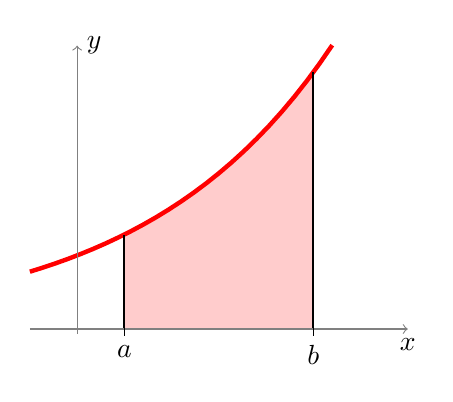
\begin{tikzpicture}[scale=1.2,xscale=2]
  \fill[red!20,] (0,0) -- plot[domain=0:1,smooth] (\x,{exp(\x)}) -- (1,0) -- cycle;
  \draw[ultra thick, color=red,domain=-0.5:1.1] plot (\x,{exp(\x)});
  \draw[thick] (0,0)--(0,1);
  \draw[thick] (1,0)--(1,2.718);


  \draw[gray,->] (-0.5,0) -- (1.5,0) node[below,black] {$x$};
  \draw[gray,->] (-0.25,-0.05) -- (-0.25,3) node[right,black] {$y$};
 %\draw (1pt,1cm) -- (-1pt,1cm) node[anchor=east] {$1$};
   \foreach \x/\xtext in {0/a, 1/b}
  \draw (\x cm,2pt) -- (\x cm,-2pt) node[anchor=north] {$\xtext$};
\end{tikzpicture}\quad
\begin{tikzpicture}[scale=1.2,xscale=2]
\rectangleexp{5}
\end{tikzpicture}\quad
\begin{tikzpicture}[scale=1.2,xscale=2]
\rectangleexp{10}
\end{tikzpicture}
\end{center}

\begin{minipage}{0.6\textwidth}
Un rectangle élémentaire entre $x$ et $x+\dd x$ a pour base $\dd x$ (où $\dd x$ désigne ici un élément infinitésimal) et pour hauteur $f(x)$ donc son aire vaut $f(x) \times \dd x$. 
Ainsi l'aire sous la courbe est approchée par une somme de termes $f(x)\dd x$, pour $x$ variant de $a$ à $b$. Cette somme est notée $\int_a^b f(x)\,\dd x$.
Le symbole $\int$ étant un $S$ allongé (pour \emph{S}omme).
\end{minipage}\qquad
\begin{minipage}{0.29\textwidth}
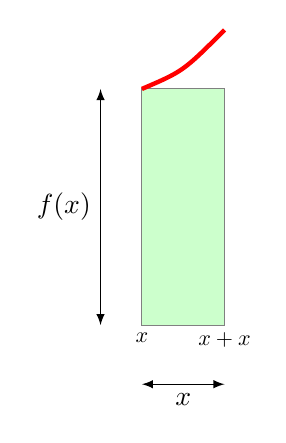
\begin{tikzpicture}[scale=1.5,xscale=0.7]
% Rectangle a gauche (en vert)
 \filldraw[fill=green!20,draw=gray] (1,0)--(1,2)--(2,2)--(2,0)--cycle;
 \draw[ultra thick, color=red] (1,2).. controls (1.5,2.15) ..  (2,2.5);
 \node[below,scale=0.8] at (1,0) {$x$};
% \node[below=2ex] at (1.5,0) {$\dd x$};
 \node[below,scale=0.8] at (2,0) {$x+\dd x$};
 \draw[<->,>=latex] (0.5,0)--+(0,2) node[midway,left] {$f(x)$};
 \draw[<->,>=latex] (1,-0.5)--+(1,0) node[midway,below] {$\dd x$};
% \node[right] at (2,2.5) {$f(b)$};
\end{tikzpicture}
\end{minipage}

\begin{minipage}{0.6\textwidth}
\textbf{Exemple.}

$$\int_0^3 x\;\dd x
= \text{ aire du triangle} 
= \frac{\text{base} \times \text{hauteur}}{2}
= \frac92$$
\end{minipage}\qquad
\begin{minipage}{0.29\textwidth}
	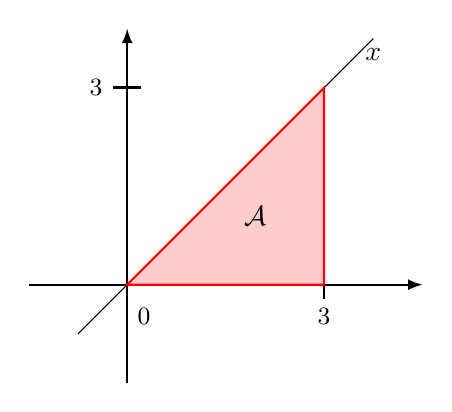
\begin{tikzpicture}[scale=2.5]
	\draw[thick,->,>=latex] (-0.5,0)--(1.5,0); % node[above] {$x$};
	\draw[thick] (0,2pt) -- (0,-2pt)node[below right] {\small$0$};
	\draw[thick] (1,2pt) -- (1,-2pt)node[below] {\small$3$};
	\draw[thick,->,>=latex] (0,-0.5)--(0,1.3); % node[above] {$y$};
	\draw[very thick] (2pt,1) -- (-2pt,1)node[left] {\small$3$};

	\draw[] (-0.25,0-0.25) -- (1.25,1.25) node[below]{$x$};
	\filldraw[thick,red,fill=red!20] (0,0) -- (1,1) -- (1,0) -- cycle;

	\draw[color=red,thick] (1,1) -- (1,0);
	% \draw[color=red,dashed] (0.5,0.25) -- (0.5,0);
	\draw (0.65,0.35) node{$\mathcal{A}$};
	\end{tikzpicture}
\end{minipage}





\begin{minipage}{0.5\textwidth}
\shorthandoff{?;:!}
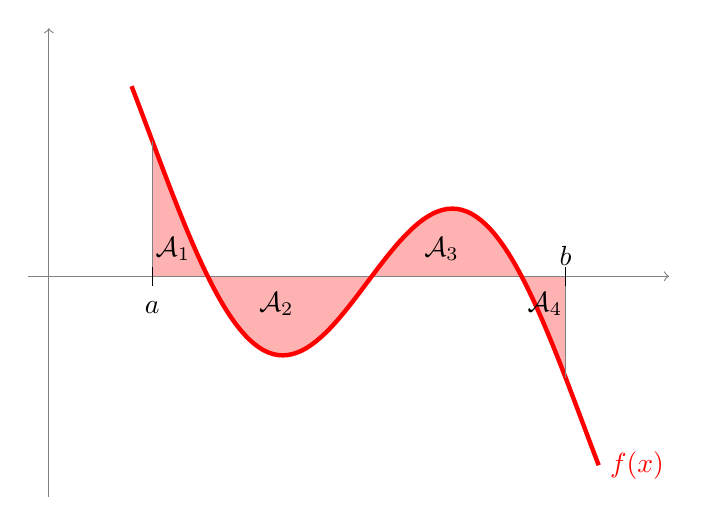
\begin{tikzpicture}[scale=3.5,xscale=1.5]
\tikzset{
	declare function={
		qcq(\t) = 0.5 - \t - 0.5*sin(6*(\t+1.05) r);
	}
}

 % tracé de la courbe et des axes
  \fill[red!30] (0,0) -- plot[domain=0:1] (\x,{qcq(\x)}) -- (1,0) -- cycle;

  \draw[gray,->] (-0.30,0) -- (1.25,0); % node[below,black] {$x$};
  \draw[gray,->] (-0.25,-0.8) -- (-0.25,0.9);% node[right,black] {$y$};

  % tracé de la courbe par-dessus les rectangles
   \draw[ultra thick, color=red,domain=-0.05:1.08, samples=100] plot (\x,{qcq(\x)}) node[right] {$f(x)$};
   \pgfmathparse{qcq(0)}   \let\y\pgfmathresult
   \draw[gray] (0,0) -- (0,\y);
   \pgfmathparse{qcq(1)}   \let\y\pgfmathresult
   \draw[gray] (1,0) -- (1,\y);

% du texte
  \draw (0 cm,1pt) -- (0 cm,-1pt) node[below=2pt] {$a$};
  \draw (1 cm,1pt) -- (1 cm,-1pt) node[above=4pt] {$b$};

  \node at (0.05,0.1) {$\mathcal{A}_1$};
  \node at (0.3,-0.1) {$\mathcal{A}_2$};
  \node at (0.7,0.1) {$\mathcal{A}_3$};
  \node at (0.95,-0.1) {$\mathcal{A}_4$};
\end{tikzpicture}
\shorthandoff{?;:!}
\end{minipage}
\begin{minipage}{0.5\textwidth}
\textbf{Signe.}
L'intégrale compte les aires avec un signe \og{}$+$\fg{} ou \og{}$-$\fg{}. Les aires sous l'axe des abscisses sont comptées négativement.
Si on note $\mathcal{A}_i>0$ les aires ci-contre, alors
$$\int_a^b f(x)\,\dd x = \mathcal{A}_1 - \mathcal{A}_2 + \mathcal{A}_3 - \mathcal{A}_4$$
\end{minipage}

%%%%%%%%%%%%%%%%%%%%%%%%%%%%%%%%%%%%%%%%%%%%%%%%%%%
\subsection*{Propriétés de l'intégrale.}


\begin{itemize}
  \item L'intégrale est \textbf{linéaire} :
\mybox{$\displaystyle\int_a^b f(x) + g(x) \; \dd x
= \int_a^b f(x) \; \dd x \  + \int_a^b g(x) \; \dd x \qquad \text{ et } \qquad 
\int_a^b k \cdot f(x)  \; \dd x = k \int_a^b f(x) \; \dd x$}

  \item La relation de Chasles est vérifiée :
\mybox{$\displaystyle\int_a^b f(x)\;\dd x = \int_a^c f(x)\;\dd x \ + \int_c^b f(x)\;\dd x$}

Avec 
$\int_a^a f(x) \;\dd x=0 \qquad \text{ et }  \quad \int_b^a f(x) \;\dd x= -\int_a^b f(x) \; \dd x.$
  
%  \item La propriété suivante s'appelle la \textbf{positivité de l'intégrale} :
% Si \quad $f(x)\ge 0$ pour tout $x\in[a,b]$ alors $\displaystyle \int_a^bf(x)\;dx \ge 0$.
\end{itemize}

\bigskip

\textbf{Exemple.}
$$\int_0^{\frac\pi4} 2xe^x - 7 \cos(x) \; \dd x
= 2\int_0^{\frac\pi4} xe^x  \; \dd x 
\ - \ 7 \int_0^{\frac\pi4}\cos(x) \; \dd x$$
Ainsi la linéarité permet de se ramener au calcul d'intégrales plus simples.
(On verra dans les autres fiches comment calculer ces intégrales.)

\bigskip

\textbf{Exemple.}
Comment calculer $\int_3^5 x \; \dd x$ ?

\begin{minipage}{0.45\textwidth}
On peut utiliser la relation de Chasles sur les bornes : 
$$ \underbrace{\int_0^5 x \; \dd x}_{\text{aire du triangle $T$}} =  
\underbrace{\int_0^3 x \; \dd x}_{\text{aire du triangle $T'$}}
+ \underbrace{\int_3^5 x \; \dd x}_{\mathcal{A}}$$
\end{minipage}\qquad\qquad
\begin{minipage}{0.5\textwidth}
	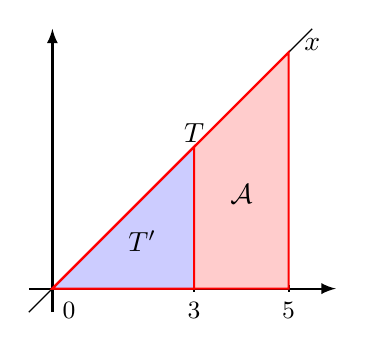
\begin{tikzpicture}[scale=.6]
	\draw[thick,->,>=latex] (-0.5,0)--(6,0); % node[above] {$x$};
	\draw[thick] (0,2pt) -- (0,-2pt)node[below right] {\small$0$};
	\draw[thick] (3,2pt) -- (3,-2pt)node[below] {\small$3$};
	\draw[thick] (5,2pt) -- (5,-2pt)node[below] {\small$5$};

	\draw[thick,->,>=latex] (0,-0.5)--(0,5.5); % node[above] {$y$};
	%\draw[very thick] (2pt,1) -- (-2pt,1)node[left] {\small$3$};

	\draw[] (-0.5,0-0.5) -- (5.5,5.5) node[below]{$x$};
	\filldraw[thick,red,fill=red!20] (0,0) -- (5,5) -- (5,0) -- cycle;
	\filldraw[thick,red,fill=blue!20] (0,0) -- (3,3) -- (3,0) -- cycle;

	% \draw[color=red,thick] (1,1) -- (1,0);
	% \draw[color=red,dashed] (0.5,0.25) -- (0.5,0);
	\draw (3,3.3) node{$T$};
	\draw (1.9,1) node{$T'$};
    \node at (4,2) {$\mathcal{A}$};
	\end{tikzpicture}
\end{minipage}

Ainsi en utilisant la formule $\frac{\text{base} \times \text{hauteur}}{2}$ pour calculer l'aire des deux triangles, on a :
$$\frac{5 \times 5}{2} = \frac{3 \times 3}{2} + \mathcal{A}.$$
Ainsi
$$\mathcal{A} = \int_3^5 x \; \dd x = \frac{25}{2} - \frac92 = \frac{16}{2}=8.$$

\emph{Exercice.} Retrouver cette aire en utilisant la formule générale de l'aire d'un trapèze.
 
\begin{minipage}{0.64\textwidth}
$$\mathcal{A} = \frac{(\text{petite base}+\text{grande base})}{2} \times \text{hauteur} = \frac{(b+B)}{2}\times h$$
\end{minipage}
\begin{minipage}{0.3\textwidth}
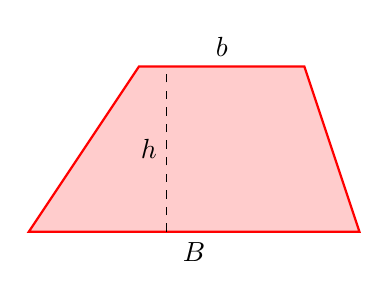
\begin{tikzpicture}[scale=0.7]
  \filldraw[thick,red,fill=red!20]
(0,0) to node[midway,below,black]{$B$}  (6,0) to (5,3) tonode[midway,above,black]{$b$} (2,3) -- cycle;

  \draw[dashed] (2.5,0) -- +(0,3) node[midway,left]{$h$};
\end{tikzpicture}
\end{minipage}



\end{document}